% Description: TD de programmation sous SIG - Arcpy (module principal)

% Modules generaux
\documentclass[11pt]{article}
\usepackage[utf8]{inputenc}
\usepackage[T1]{fontenc}
\usepackage[francais]{babel} % prise en charge du francais
\usepackage[table]{xcolor} % tableaux
\usepackage{graphicx} % images
\usepackage{float}
\usepackage[font=small]{caption}

% Marges
\usepackage[left=2cm,right=2cm,top=2cm,bottom=2cm]{geometry}

% Personnalisation des titres
\usepackage{titlesec}
\titlespacing{\section}{0em}{4em}{1em}
\titlespacing{\subsection}{0em}{2em}{0em}
\titlespacing{\subsubsection}{0em}{0.5em}{0em}

% Mise en page
\setlength{\parskip}{1.2em}
\renewcommand{\floatpagefraction}{1}

% Couleurs personnalisées
\usepackage{color}
\definecolor{lightgray}{gray}{0.98}
\definecolor{gray}{rgb}{0.6, 0.6, 0.65}
\definecolor{green}{rgb}{0.133, 0.545, 0.133}
\definecolor{blue}{rgb}{0, 0, 1}
\definecolor{red}{rgb}{0.6, 0.1, 0.1}

% Liens hypertextes
\usepackage{hyperref}
\hypersetup{
	colorlinks=true,
	breaklinks=true,
	urlcolor=blue,
	linkcolor=blue,
	pdfborder=000,
	pdftex=true
}

% Mise en forme des codes python
\usepackage{fancyvrb}  % modification de la taille de la police dans un environnement verbatim
\usepackage{listingsutf8}
\lstset{
	language=python,
	inputencoding=utf8/latin1,
	extendedchars=true,
	keywordstyle=\bfseries\ttfamily\color{blue},
	identifierstyle=\ttfamily,
	commentstyle=\color{gray},
	stringstyle=\ttfamily\color{green},
	showstringspaces=false,
	basicstyle=\footnotesize\ttfamily,
	tabsize=2,
	breaklines=true,
	extendedchars=true,
	xleftmargin=1cm, 
	xrightmargin=1cm,
	backgroundcolor=\color{lightgray},
	literate=%
		{é}{{\'{e}}}1
		{è}{{\`{e}}}1
		{ê}{{\^{e}}}1
		{ë}{{\¨{e}}}1
		{û}{{\^{u}}}1
		{ù}{{\`{u}}}1
		{â}{{\^{a}}}1
		{à}{{\`{a}}}1
		{î}{{\^{i}}}1
		{ô}{{\^{o}}}1
		{ç}{{\c{c}}}1
}

% Commandes personnalisées
\newcommand{\bslash}{\texttt{\symbol{92}}}
\newcommand{\action}{$\Rightarrow$ }
\newcommand{\reponse}{
	\begin{tabbing}
	\hspace{2cm}\=\kill
	Réponse \> ............................................................................................ \\ 
 	\> ............................................................................................
	\end{tabbing}
}

\newenvironment{note}{%
	\begin{tabular}[t t]{c c}
		
\includegraphics{img/tips.png}
		 &
		\begin{minipage}[c]{0.9\linewidth}
			\begin{sffamily}
}{%
			\end{sffamily}
		\end{minipage}
	\end{tabular}	
}

\newsavebox{\mybox}
\newenvironment{objectifs}{
	\begin{lrbox}{\mybox}
		\begin{minipage}{0.9\textwidth}
			\vspace{1em}
			\begin{tabular}[t t]{c c}
				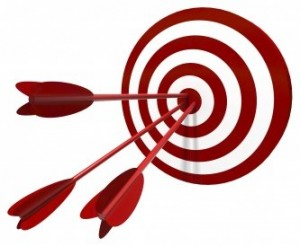
\includegraphics[width=0.1\linewidth]{img/goals.jpg} &
				\begin{minipage}[c]{0.8\linewidth}
					\hspace{2em}\textbf{\large{Objectifs :}} \\
}{
				\end{minipage}
			\end{tabular}
			\vspace{1em}
		\end{minipage}
	\end{lrbox}
	\fbox{\usebox{\mybox}}
}

\newcommand{\code}[1]{\lstinline{#1}}

\newenvironment{python}{%
	\begin{lstlisting}
}{%
	\end{lstlisting}
}


%%%%%%%%%%%%%%%%%%%%%%%%%%%%%%%%%
% Infos générales sur le document
%%%%%%%%%%%%%%%%%%%%%%%%%%%%%%%%%
\title{Arcpy (module principal)}
\author{Clément Delgrange}
\date{\today}

% Entetes et pieds de page
\usepackage{fancyhdr}
\pagestyle{fancy}
\fancyhf{}
\renewcommand{\headrulewidth}{0pt}
\makeatletter
\fancyfoot[L]{ENSG}
\fancyfoot[C]{-\thepage-}
\fancyfoot[R]{\@title}
\makeatother
\renewcommand{\footrulewidth}{0.5pt}


%%%%%%%%%%%%
%%% Document
%%%%%%%%%%%%
\begin{document}
\parindent=0cm

\makeatletter
\begin{center}
	\hrule
	\vspace{1em}
	{\small \textit{Programmation sous SIG}}\\	
	\vspace{0.5em}
	{\Large \bfseries{\@title}}
	\vspace{1em}
	\hrule
\end{center}
\makeatother



\begin{objectifs}
\begin{itemize}
	\item savoir parcourir une arborescence, un espace de travail
	\item être capable de vérifier qu'un jeu de données existe
\end{itemize}
\end{objectifs}




\section*{Préalables}
Franc'O est un organisme chargé de la collecte et de la diffusion des données de nature hydrographique sur l'ensemble du territoire français. L'organisme est organisé en zones de collectes au sein desquelles un agence locale effectue des saisies de données géographiques. L'ensemble des données sont ensuite centralisée au siège de l'organisme à Paris.

Malheureusement, les erreurs de livraison sont fréquentes. Aussi avant d'intégrer les données des agences locales, le siège parisien effectue un ensemble de contrôle sur les données reçues.

Les données sont échangées sous forme de géodatabases Esri. En fonction des anomalies détectées, les lots sont corrigés ou renvoyés en région pour correction.

En bout de chaîne, après avoir intégré les données à la base nationale et effectué divers des analyses Franc'O redistribue les données sous forme de shapefiles aux communes qui en font la demande.

Nous sommes chargées de l'automatisation des chaînes de contrôle et d'export des données. 

\begin{note}
Les ressources suivantes vous seront utiles pour réaliser ce TD. N'hésitez pas à les consulter.
\begin{itemize}
	\item \textit{Memo ArcPy} du cours de programmation sous SIG.
	\item Doc d'ArcPy : \url{http://desktop.arcgis.com/fr/arcmap/lastest/analyze/arcpy}
\end{itemize}
\end{note}

\action Quels types de développements vous paraissent pertinents pour réaliser l'automatisation des chaînes de traitement de Franc'O ?

\reponse

% Pas de "bonne" réponse : la question est là pour amener l'étudiant à réfléchir à ce qu'il va faire.
% Pour la correction, nous utiliserons un script python autonome.

\section{Contrôle des géodatabases}

La structure attendue des géodatabases est décrite à l'aide du dictionnaire Python de la forme suivante :
\begin{lstlisting}
DICO_GDB_STRUCT = {
    "ADMINISTRATIF": {
        "COMMUNE": {
            "NOM": ["String", 50],
            "CODE_INSEE": ["Integer", 5],
            "STATUT": ["String", 200]
        }
    },
    "HYDROGRAPHIE": {
        "COURS_D_EAU": {
            "CODE_HYDRO": ["String", 8],
            "CLASSE": ["String", 1],
            "TOPONYME": ["String", 127],
            "REGIME": ["String", 50]
        }
    }
}
\end{lstlisting}

Il se lit de la manière suivante : le jeu de classes d'entités \code{ADMINISTATIF} contient une classe d'entités \code{COMMUNE} possédant trois champs : \code{NOM}, de type \code{String} et de longueur 50,   \code{CODE_INSEE}, de type \code{Integer} et de longueur 5, et \code{STATUT}, de type \code{String} et de longueur 200, etc.

Les résultats du contrôle doivent être écrits dans un fichier de log. Les informations y sont rangées en fonction de leur importance. Trois niveaux seront utilisés :
\begin{itemize}
	\item les erreurs (importance = 3) :
	\begin{itemize}
		\item jeux de classes d'entités et classes d'entités en manquants;
		\item pour chaque classe d'entités, champs manquants;
		\item pour chaque champ, type et/ou longueur incorrects;
	\end{itemize}
	\item les erreurs non bloquantes (importance = 2) :
	\begin{itemize}
		\item jeux de classes d'entités et classes d'entités en trop;
		\item pour chaque classe d'entités, champs en trop;
	\end{itemize}
	\item les simples informations (importance = 1) :
	\begin{itemize}
		\item jeux de classes d'entités et classes d'entités présents;
		\item pour chaque classe d'entités, champs présents;
	\end{itemize}
\end{itemize}

Le log aura finalement la forme suivante : 
\begin{Verbatim}[fontsize=\scriptsize]
24/08/17 18:10:56 : Début des contrôles
Chemin de la géodatabase : D:\ProgSIG\TD4\data\BaseHydro.gdb

[Info]		Jeu de classes d'entités ADMINISTRATIF présent dans la géodatabase
[Info]		Classe d'entités COMMUNE présente dans le jeu de classes d'entités ADMINISTRATIF
[Info]		Champ NOM présent dans la table COMMUNE
[ERREUR]	Longueur du champ NOM de la table COMMUNE incorrect (attendu : 50, obtenu : 45)
[Info]		Champ CODE_INSEE présent dans la table COMMUNE
[ERREUR]	Type du champ CODE_INSEE de la table COMMUNE incorrect (attendu : Integer, obtenu : String)
[Info]		Champ STATUT présent dans la table COMMUNE
[Attention]	Champ POPUL (Integer, 4) non requis dans la table COMMUNE
[Attention]	Classes d'entités TRONCON_HYDRO non requise dans le jeu de classes d'entités ADMINISTRATIF

24/08/17 18:11:01 Fin des contrôles
Nombre d'erreurs : 2
\end{Verbatim}

\action Dans un script Python, écrivez une fonction \code{write_log(msg, flog, importance=0)} écrivant le message \code{msg} dans un fichier texte \code{flog} avec une importance \code{importance}.

\action Développez un utilitaire permettant de détecter les jeux de classes d'entités et classes d'entités absents de la géodatabase alors qu'ils y sont attendus. Vous utiliserez la fonction précédente pour écrire les résultats dans un fichier texte.

\action Complétez votre programme précédent en ajoutant le contrôle des champs (présents, absents, type et longueur).

\begin{note}
N'hésitez pas à découper votre code en fonctions pour le rendre plus clair et plus facilement maintenable !
\end{note}

\action Enfin ajoutez un dernier contrôle permettant de détecter les jeux de classes d'entités et classes d'entités en trop dans la géodatabase.



\section{Export des données}

\action En partant de la géodatabase correcte, développez un outil permettant d'exporter les données d'une commune. L'outil demande le numéro INSEE de la commune et génère quatre shapefiles (un pour chacune des classes d'entités de la géodatabase) contenant les données intersectant le territoire de la commune.


\end{document}
